\documentclass[12pt,a4paper]{article}
\usepackage[T1]{fontenc}
\usepackage[utf8]{inputenc}
\usepackage[english]{babel}
\usepackage{mathptmx}
\usepackage[a4paper,margin=2.5cm,headheight=16pt]{geometry}
\usepackage{graphicx,caption,booktabs,tabularx,enumitem}
\usepackage{tikz}
\usetikzlibrary{arrows.meta,positioning,shapes.geometric}
\usepackage{xcolor}
\definecolor{baslik}{HTML}{17365D}
\usepackage{titlesec}
\titleformat{\section}{\Large\bfseries\color{baslik}}{\thesection}{.7em}{}
\titleformat{\subsection}{\large\bfseries\color{baslik}}{\thesubsection}{.7em}{}
\titlespacing*{\section}{0pt}{1.4ex plus .2ex}{.7ex}
\usepackage{fancyhdr,lastpage}
\pagestyle{fancy}\fancyhf{}


\newcommand{\ogrenciad}{Kaan Karaali}
\newcommand{\ogrencino}{Public portfolio}

\fancyhead[L]{\small \ogrenciad\enspace--\enspace\ogrencino}
\fancyhead[R]{\small EHB326E}

\fancyfoot[C]{\thepage\ / \pageref{LastPage}}
\renewcommand{\headrulewidth}{0.4pt}
\usepackage{ragged2e}
\AtBeginDocument{\justifying}
\usepackage{hyperref}
\hypersetup{colorlinks=true,linkcolor=baslik,urlcolor=baslik,citecolor=baslik}

\newcommand{\raporbasligi}{Implementation and Simulation of the uBee SoC in Vivado}

\begin{document}
\begin{center}
{\Large\bfseries Istanbul Technical University}\\[3pt]
{\large EHB326E -- Homework 1 Report}\\[10pt]
{\LARGE\bfseries\color{baslik}\raporbasligi}\\[8pt]
\ogrenciad\quad(\ogrencino)\\[3pt]
\today
\end{center}
\vspace{.3em}
\section{Abstract}
In this homework, I built the system given in Chapter~2 with the uBee RV32IMC
SoC in Vivado. I connected the processor to an AXI UART Lite block using AXI
SmartConnect. I also made the clock, reset, memory and interrupt connections.
Then I ran a behavioral simulation. The processor ran the program in its
instruction memory and sent the expected message from the UART output.

\section{Objective and Requirements}
The purpose of the homework was to build a small embedded system around the
uBee processor and check that it works. The system uses a 100~MHz input clock,
reset logic, AXI UART Lite and the given interrupt-ordering module. I used the
given \texttt{imem.hex} and \texttt{dmem.hex} files to initialize the
instruction and data memories. I checked the result by observing the UART
output in simulation.

\section{Method and System Design}
The main data path is shown in Figure~\ref{fig:system}. uBee is the AXI master
and AXI UART Lite is the slave. AXI SmartConnect connects these two blocks and
directs the processor's transactions to the UART. The base address of the UART
is \texttt{0x60000000}. When the processor writes a byte to the UART transmit
register, the UART sends that byte serially on \texttt{uart\_txd}.

\begin{figure}[htbp]\centering
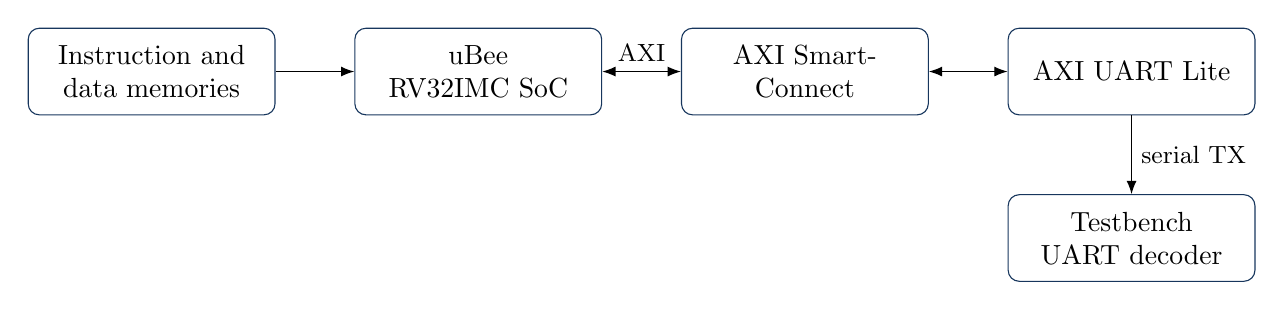
\begin{tikzpicture}[node distance=10mm and 10mm, >=Latex,
 block/.style={draw=baslik,rounded corners,align=center,minimum height=11mm,text width=29mm}]
\node[block] (memory) {Instruction and data memories};
\node[block,right=of memory] (cpu) {uBee RV32IMC SoC};
\node[block,right=of cpu] (axi) {AXI SmartConnect};
\node[block,right=of axi] (uart) {AXI UART Lite};
\node[block,below=of uart] (tb) {Testbench UART decoder};
\draw[->] (memory)--(cpu);
\draw[<->] (cpu)--node[above]{\small AXI}(axi);
\draw[<->] (axi)--(uart);
\draw[->] (uart)--node[right]{\small serial TX}(tb);
\end{tikzpicture}
\caption{Main data path used to produce and verify the UART message.}
\label{fig:system}
\end{figure}

The Clocking Wizard generates the system clock. Its \texttt{locked} output
shows that the clock is stable. Processor System Reset keeps the other blocks
in reset until the clock is ready. I connected the UART interrupt to input~0
of the interrupt-ordering module. I tied the other 15 inputs to zero and
connected its 16-bit output to the processor's external interrupt input. This
test only checks UART transmission, so the interrupt is connected but not
tested by the program.

\section{Simulation and Results}
The testbench generated the 100~MHz clock and kept the design in reset at the
beginning. After reset was released, the processor started fetching and
executing instructions. The testbench watched \texttt{uart\_txd} and decoded
the UART frames at 9600 baud. It collected the received characters and
compared them with the expected message. This is needed because
\texttt{uart\_txd} carries one serial bit at a time.

\begin{table}[htbp]\centering
\caption{Behavioral simulation observations}\label{tab:test}
\begin{tabularx}{\linewidth}{@{}lXXX@{}}\toprule
Test & Condition & Expected result & Observed result \\ \midrule
Reset & Reset asserted, then released & Processor starts from initialized instruction memory & Instruction execution started after reset \\
UART TX & Supplied program executed at 100~MHz & ``Hello from uBee on Arty A7'' is transmitted at 9600 baud & Complete message decoded; testbench reported PASS \\ \bottomrule
\end{tabularx}
\end{table}

Figure~\ref{fig:uartwave} shows the serial transmit signal and the characters
decoded by the testbench. The values of \texttt{char\_byte} form the expected
message and \texttt{fail\_q} stays at zero.

\begin{figure}[htbp]\centering
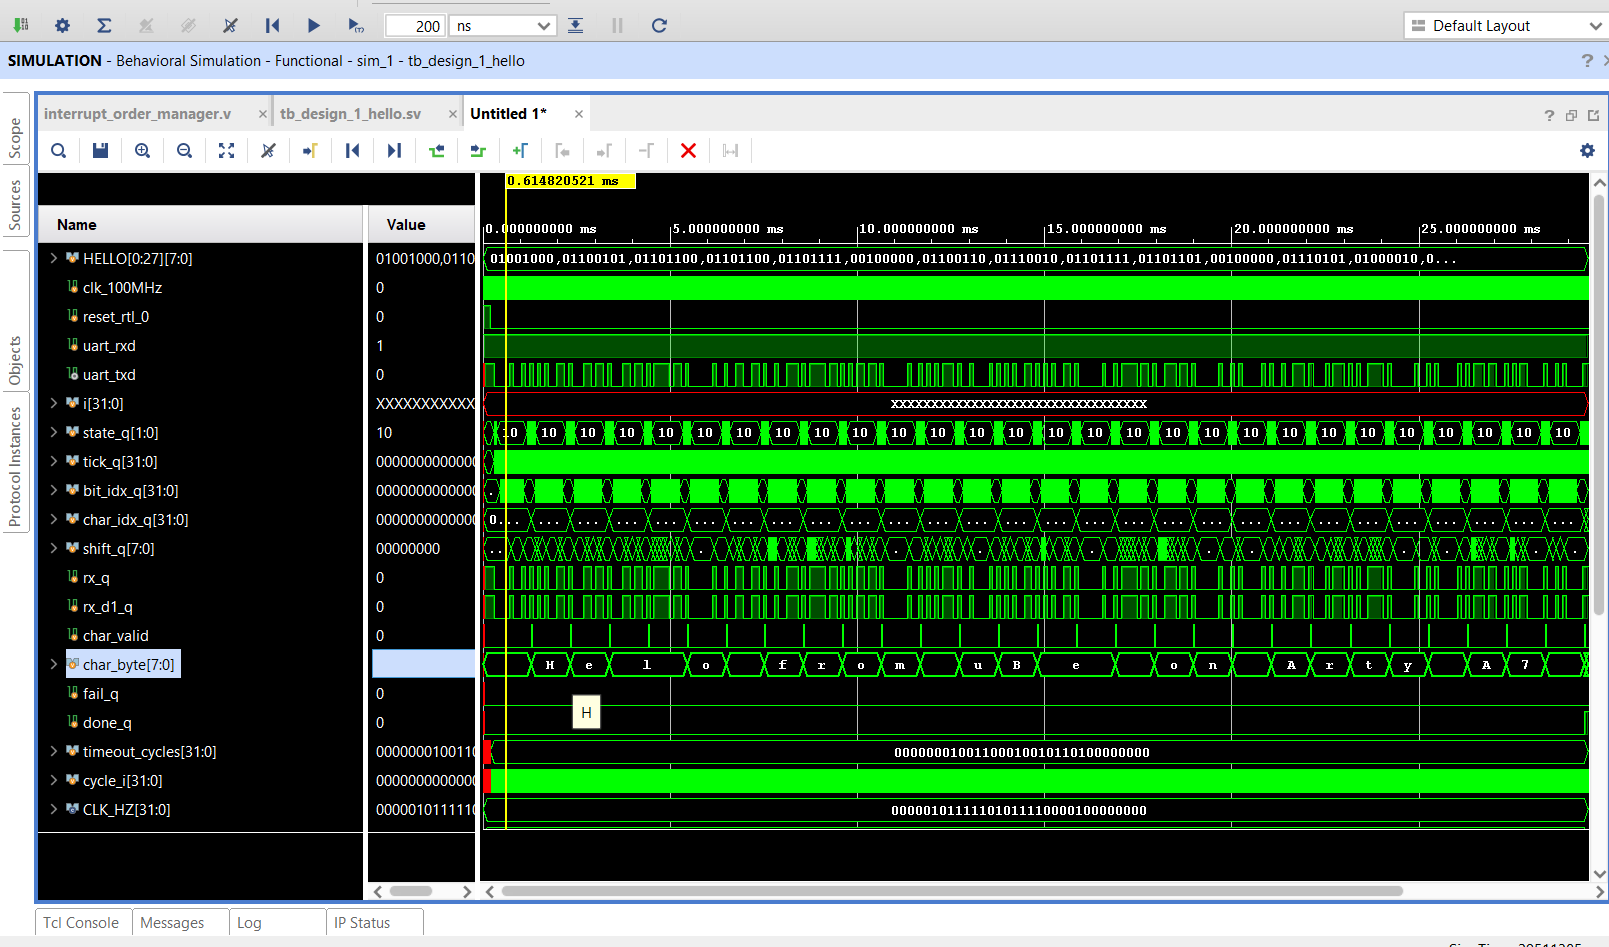
\includegraphics[draft=false,width=.72\linewidth]{../evidence/simulation_waveform.png}
\caption{UART transmit waveform and characters decoded by the testbench.}
\label{fig:uartwave}
\end{figure}

The decoded text was ``Hello from uBee on Arty A7''. At the end, the testbench
printed \texttt{PASS: tb\_design\_1\_hello}. The simulation finished at about
29.51~ms. This time is reasonable for sending 28 characters at 9600 baud when
the start and stop bits are also included.

\section{Verification and Evaluation}
The result in Table~\ref{tab:test} shows that the instruction memory, processor,
AXI connection and UART transmit path worked together. The processor also
started correctly after reset. UART reception and interrupt handling were not
tested because \texttt{uart\_rxd} stayed idle during this simulation.

\section{Conclusion}
I completed the uBee system in Vivado and tested it with behavioral simulation.
The processor ran the supplied program and sent the correct message through
AXI UART Lite. The testbench gave a PASS result for the transmit test. UART
reception and interrupt servicing were not tested in this homework.

\begin{thebibliography}{99}
\bibitem{coursebook} EHB326E course material, \emph{Introduction to
Embedded Systems}, Chapter~2.
\bibitem{ubee} GSTL-ITU, \emph{uBee repository},
\url{https://github.com/GSTL-ITU/uBee}, accessed 5 October 2026.
\end{thebibliography}
\end{document}

